%\ctparttext{\color{black}\begin{center}
%		Esta es una descripción de la parte de informática.
%\end{center}}

%\part{Parte de informática}
\chapter{Caso 3: Personas con hipoteca, alquiler o cesión gratuita}

\section{Descripción del caso de estudio}
En este caso de estudio se han elegido las respuestas para las que el régimen de tenencia es distinto de en propiedad sin hipoteca, es decir, pueden estar en propiedad con hipoteca, en alquiler a precio de mercado o inferior o en cesión gratuita.

Se pretende estudiar las relaciones entre gastos en la hipoteca o alquiler, alimentación, número de miembros y ayudas sociales.

Las variables que se van a seleccionar para realizar el análisis son:
\begin{itemize}
\item \textbf{Renta}: Renta disponible total del hogar en el año anterior al de encuesta.
\item \textbf{Alimentos}: Durante el mes pasado, ¿cuál fue aproximadamente el importe que el hogar gastó en alimentos y bebidas no alcohólicas para ser consumidas en casa?
\item \textbf{Asistencia social}: Ingresos por asistencia social en el año anterior al
de encuesta.
\item \textbf{Gastos}: Gastos de la vivienda: Alquiler (si la vivienda se encuentra en régimen de alquiler), intereses de la hipoteca (para viviendas en propiedad con pagos pendientes) y otros gastos asociados (comunidad, agua, electricidad, gas, etc.)
\item \textbf{Número de miembros}: Número de miembros del hogar.
\end{itemize}

Este caso de estudio consta de $7295$ respuestas a la encuesta, cada una con las $5$ variables indicadas.

\section{Ejecución de algoritmos}

Las diferentes medidas obtenidas para cada algoritmo se muestran en \eqref{tab:c3_alg}.

\begin{table}[H]
\centering
\caption{Caso 3 - Resultados de ejecución de algoritmos.}
\label{tab:c3_alg}
\begin{tabular}{ccccc}
\toprule
 Algoritmo & Tiempo (s) & Silhouette & Calinski-Harabasz & Número de clusters \\
\midrule
kmeans & 0.145 & 3108.765 & 0.28264 & 5 \\
birch & 0.277 & 668.429 & 0.35988 & 5 \\
spectral & 10.964 & 2192.446 & 0.28476 & 5 \\
dbscan & 0.801 & 310.408 & 0.57966 & 2 \\
meanshift & 58.323 & 140.587 & 0.28696 & 15 \\
\bottomrule
\end{tabular}
\end{table}

Al igual que en los otros casos, meanshift sigue tardando mucho más tiempo que el resto de algoritmos, seguido por spectral cluster. Llama la atención que DBSCAN en este caso ha resultado mucho más lento que en los anteriores, aunque sigue sin llegar a un segundo. Kmeans y birch han tardado tiempos similares.

De nuevo, DBSCAN ha hecho una agrupación mala en dos clusters, el cluster $0$ con el $89.51\%$ de los objetos y los restantes en el cluster $-1$.

Meanshift ha agrupado los objetos en 15 clusters, y ha obtenido un valor de calinski-harabasz bastante bajo en comparación con los demás algoritmos, lo que hace sospechar que su agrupación no va a ser demasiado buena. Mirando el tamaño de los clusters generados ha realizado uno con el $94.67\%$ de los elementos, y el resto los ha agrupado en clusters con tamaños inferiores al $2.6\%$. Por tanto, a pesar de que su silhouette no sea especialmente bajo en comparación con los otros algoritmos, parece que el clustering ha sido bastante malo.

De entre los tres algoritmos restantes, pese a que birch tiene el mayor silhouette, su calinski-harabasz es muy bajo. Y entre kmeans y spectral clustering, dado que tienen valores de silhouette similares, a priori kmeans habría realizado mejor agrupamiento, pues su calinski-harabasz es mayor.


\section{Análisis}


Para el análisis nos basaremos en los resultados de kmeans, pues ha obtenido, en principio, los mejores resultados en la ejecución. Este algoritmo genera 5 clusters. cuatro con tamaño similar y uno más pequeño, como se puede ver en \eqref{c3_tam}

\begin{figure}[H]
\caption{Caso 3- Tamaño de los clusters generados por kmeans}
\label{c3_tam}
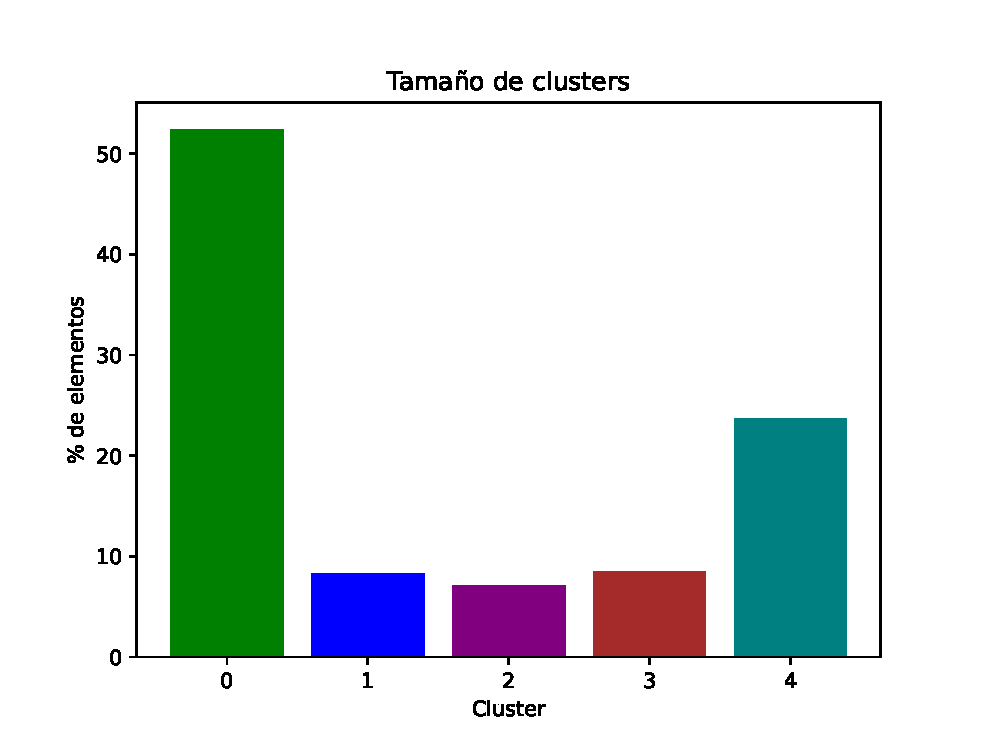
\includegraphics[scale=1]{caso3/kmeans/bar.eps}
\end{figure}

Ahora estudiamos la scatter matrix \eqref{c3_scatter}:

\begin{figure}[H]
\caption{Caso 3- Scatter matrix de kmeans}
\label{c3_scatter}
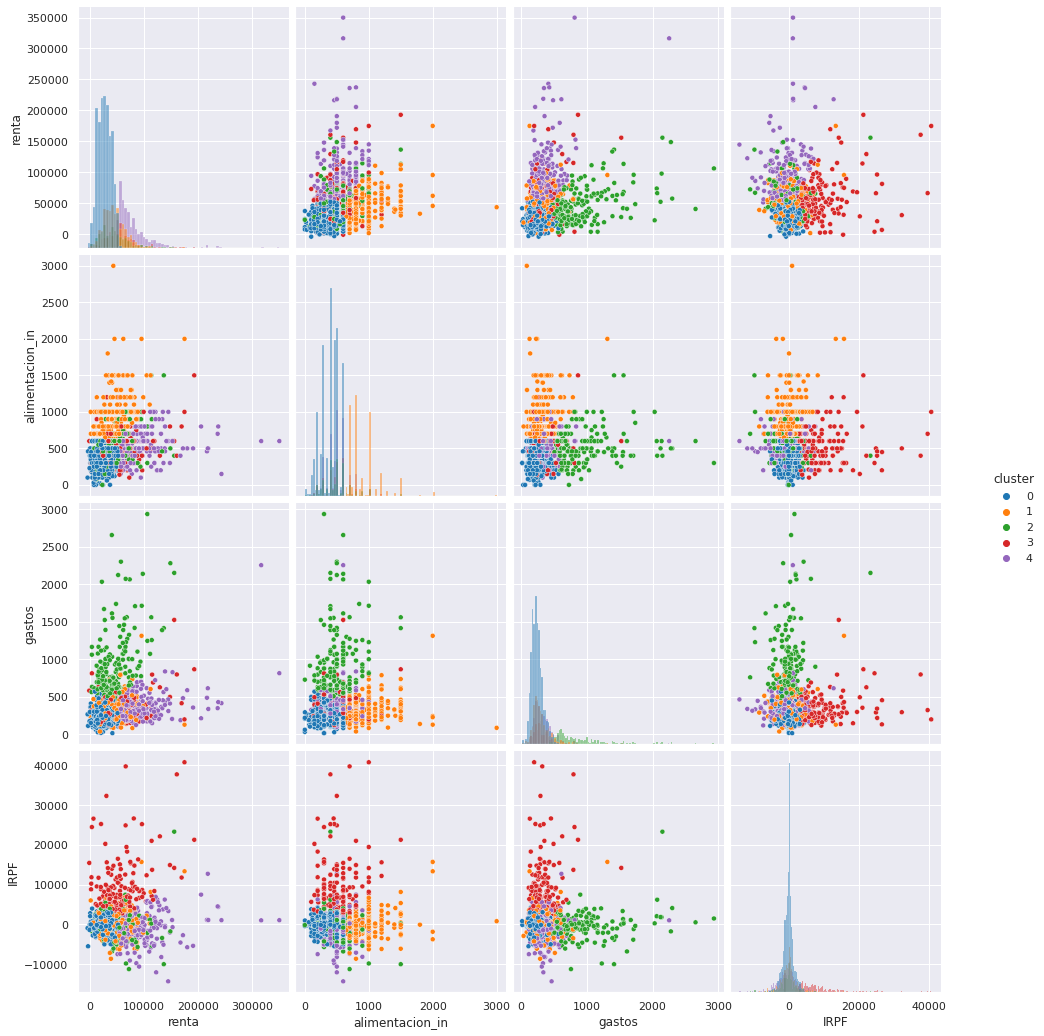
\includegraphics[scale=0.45]{caso3/kmeans/scatter.png}
\end{figure}

Analizamos \eqref{c3_scatter}, obteniendo así una distinción relativamente clara de los clusters. El cluster 2, de color verde, solo requiere una variable para identificarse, la de alimentos, mientra que los demás pueden distinguirse entre ellos usando solamente alimentos y el número de miembros del hogar.

Llama la atención sobre esta gráfica como el número de miembros, al ser una variable discreta, los puntos se encuentran alineados en los valores enteros.

\begin{figure}[H]
\caption{Caso 3- Heatmap de kmeans}
\label{c3_heatmap}
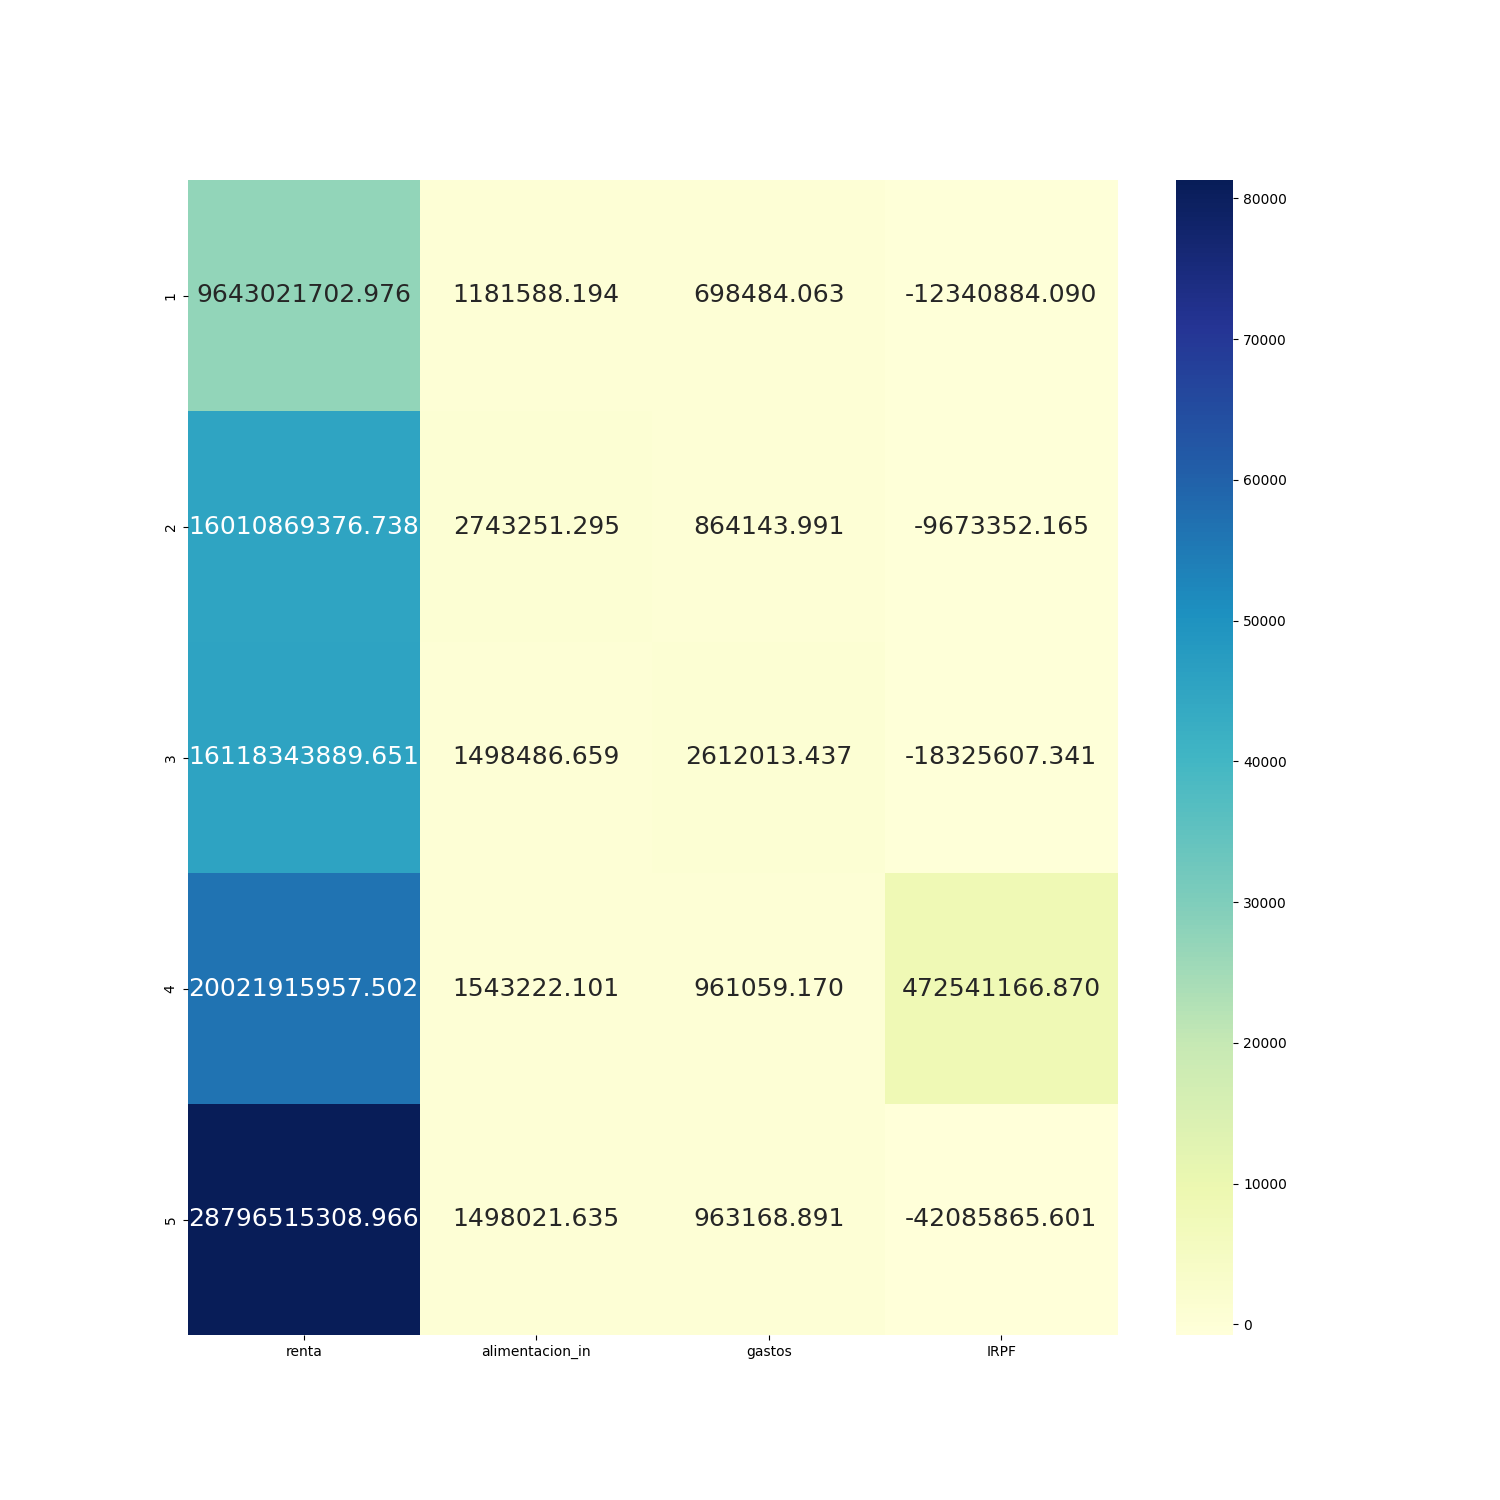
\includegraphics[scale=0.45]{caso3/kmeans/heatmap.png}
\end{figure}

En \eqref{c3_heatmap} podemos observar como el cluster 3 toma valores en general mayores en alimentos que los otros clusters.

Sin embargo, pese a que en la scatter matrix \eqref{c3_scatter} se distinguieran bien los clusters solamente usando alimentos y número de miembros, en el heatmap esta división no se ve tan clara, aunque si se aprecia que el cluster 4 (que en la scatter matrix es el 3) el número de miembros del hogar es 1. Y el cluster 5 puede distnguirse del 1, 2 y 4 usando el número de miembros, y del 3 mediante el número de alimentos.


\begin{figure}[H]
\caption{Caso 3- MDS de kmeans}
\label{c3_mds}
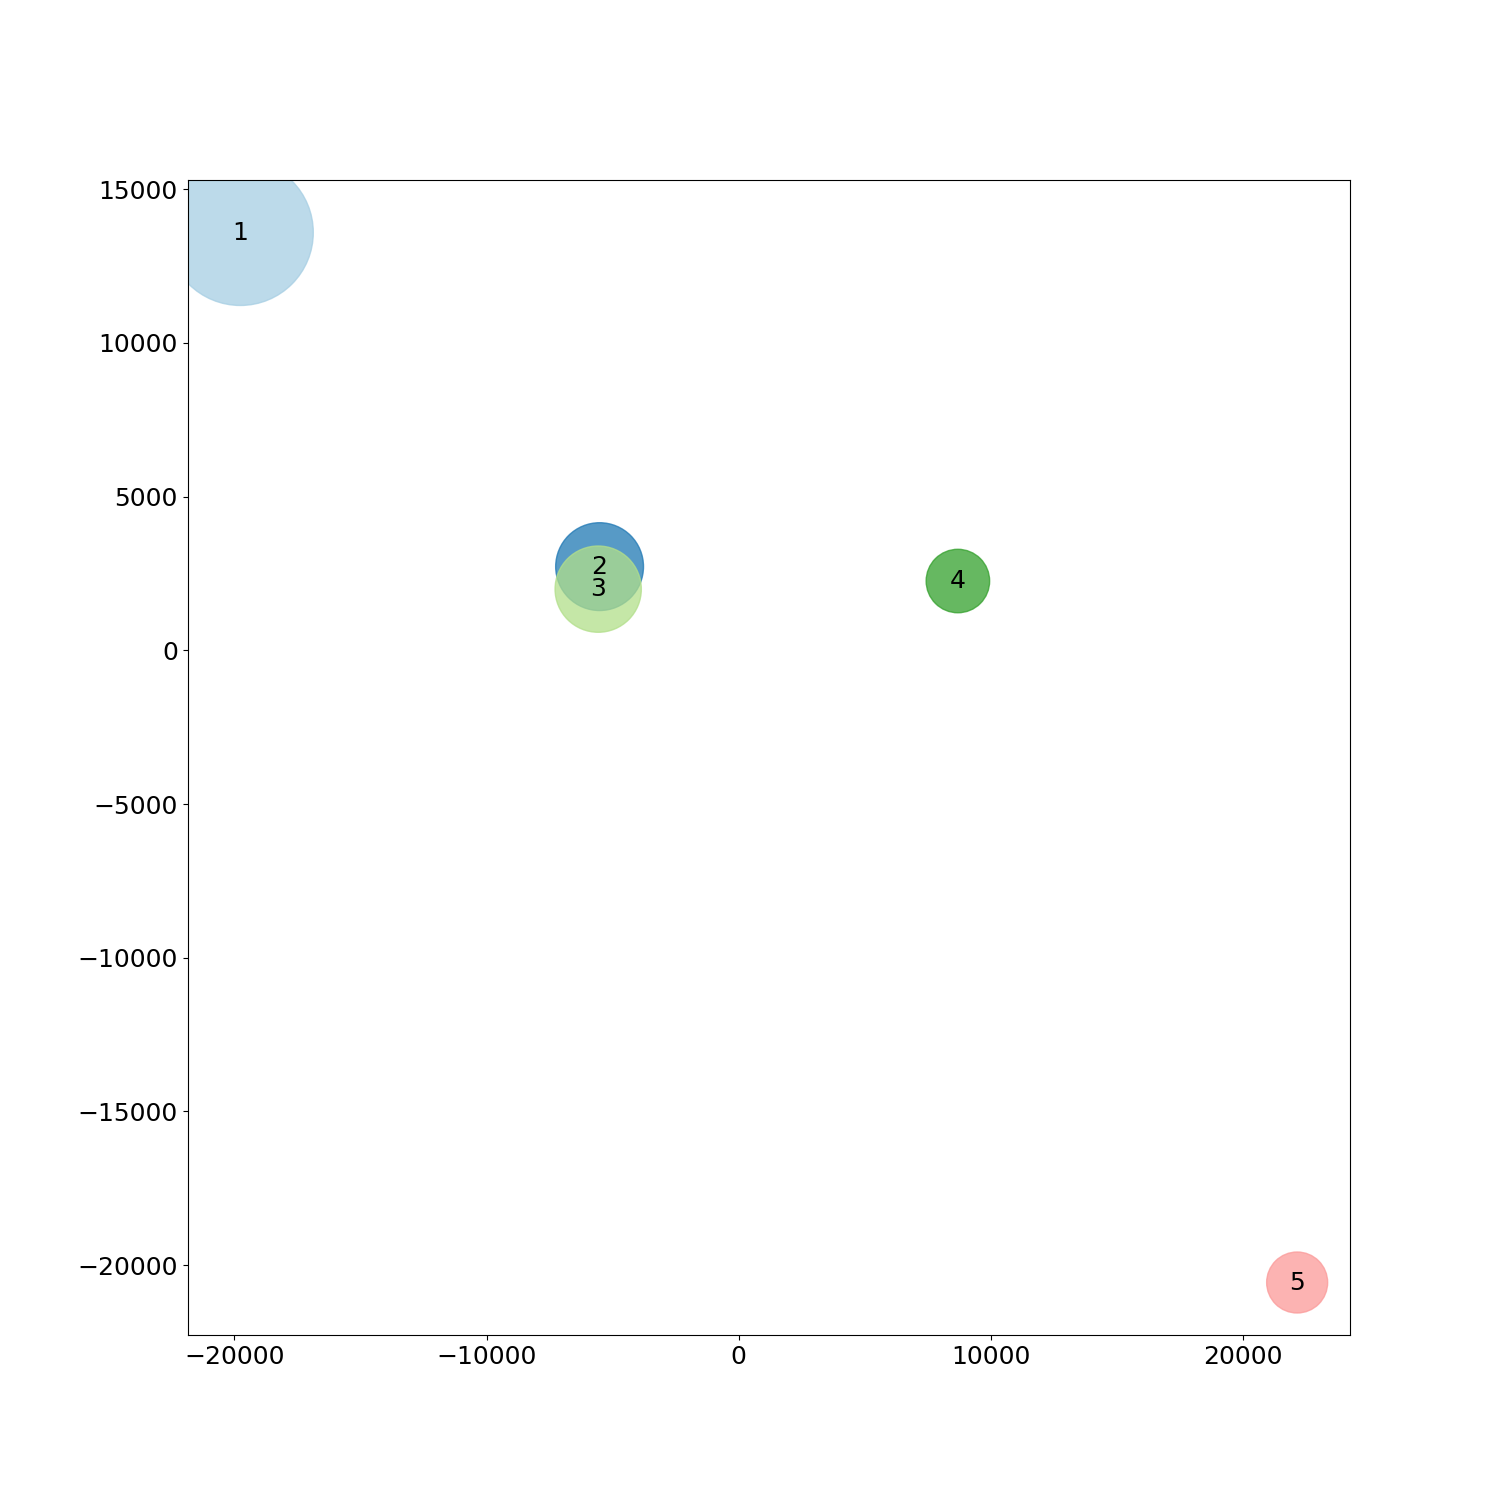
\includegraphics[scale=0.45]{caso3/kmeans/mds.png}
\end{figure}

En \eqref{c3_mds} se aprecia como los clusters están notablemente separados y con tamaños bastante similares.

\begin{figure}[H]
\caption{Caso 3- Parallel coordinates de kmean}
\label{c3_parallel}
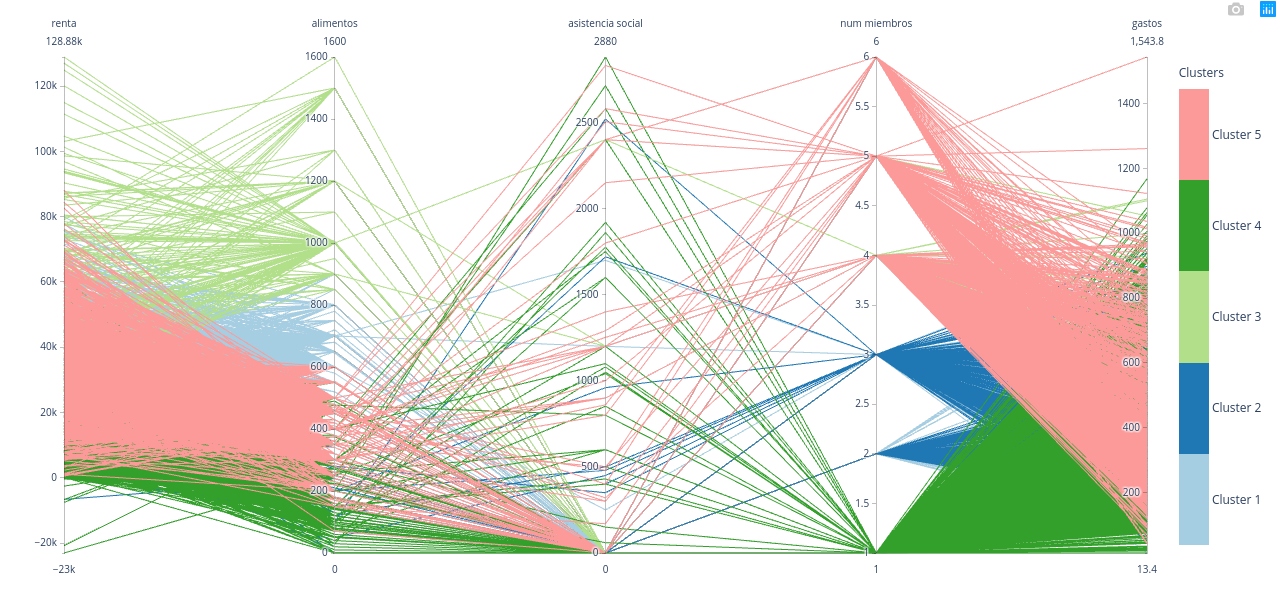
\includegraphics[scale=0.4]{caso3/kmeans/parallel.png}
\end{figure}

Finalmente, en \eqref{c3_parallel} se aprecia muy bien como el número de miembros toma valores discretos, pues se agrupan las líneas en los números enteros de esta columna. También se ve claramente como el cluster verde claro, que es el 3, toma valores mucho más altos en alimentos que el resto, aunque es algo disperso. El cluster rosa, correspondiente al 5 es menos disperso y toma valores de número de miembros más altos que los otros clusters.

Si combinamos de nuevo la información de las líneas que llegan a alimentos y número de miembros, obtenemos los mismos resultados que mediante la scatter matrix.



En la tabla  \eqref{tab:c3_variables} se muestran qué variables son necesarias para identificar cada cluster:

\begin{table}[H]
\centering
\caption{Caso 3 - Variables necesarias para separar el clustering en kmeans}
\label{tab:c3_variables}
\begin{tabular}{cccccc}
\toprule
 Cluster & renta & alimentos & asistencia social & num miembros & gastos \\
\midrule
0 & & X & & X & \\
1 & & X & & X & \\
2 & & X & & & \\
3 & & X & & X & \\
4 & & X & & X & \\
\bottomrule
\end{tabular}
\end{table}
Como se aprecia en \eqref{tab:c3_variables} con solo la variable alimentos distinguimos el cluster 2, y con alimentos y num miembros separamos los demás.

\section{Estudio de parámetros de spectral cluster}

Vamos a estudiar el comportamiento de spectral cluster variando el número de clusters que va a realizar.

\begin{table}[H]
\centering
\caption{Caso 3 - Cambio de parámetros Spectral cluster}
\label{tab:c3_spectral}
\begin{tabular}{ccccccc}
\toprule
Algoritmo & num clusters & Tiempo(s) & Silhouette & Calinski-Harabasz & n clusters \\
\midrule
spectral & 3.000 & 10.986 & 3763.346 & 0.33783 & 3 \\
spectral & 4.000 & 10.916 & 2634.019 & 0.30196 & 4 \\
spectral & 5.000 & 10.949 & 2192.446 & 0.28476 & 5 \\
spectral & 6.000 & 10.964 & 1599.167 & 0.20130 & 6 \\
spectral & 7.000 & 11.258 & 1669.853 & 0.19525 & 7 \\
spectral & 8.000 & 11.180 & 1766.949 & 0.20175 & 8 \\
spectral & 9.000 & 11.662 & 1525.245 & 0.17595 & 9 \\
spectral & 10.000 & 11.725 & 1425.793 & 0.17855 & 10 \\
\bottomrule
\end{tabular}
\end{table}

Observamos que el mayor valor de silhouette se da cuando se realizan 3 clusters, así como el mayor valor de Calinski-harabasz. Por tanto, en principio este es el mejor agrupamiento que ha realizado spectral cluster. Si miramos lso tamaños de los clusters generados vemos que son $40.11\%$, $40.08\%$ y $19.81\%$, es decir, están equilibrados dos de ellos y el tercero es algo más pequeño. No parece a priori un mal clustering.

El resto de ejecuciones de spectral cluster también genera clusters de tamaños relativamente equilibrados.

Finalmente, cabe destacar que el tiempo de ejecución se incrementa a medida que el número de clusters aumenta, pero no en una medida exagerada.


\section{Estudio de parámetros de Meanshift}

Estudiamos ahora el algoritmo Meanshift. Se ha ido variando el radio (bandwith) del algoritmo, siendo la primera entrada en la tabla el que se calcula automáticamente al ejecutar el algoritmo.

\begin{table}[H]
\centering
\caption{Caso 3 - Cambio de parámetros Meanshift}
\label{tab:c3_meanshift}
\begin{tabular}{cccccc}
\toprule
Algoritmo & bandwith & Tiempo(s) & Silhouette & Calinski-Harabasz & n clusters \\
\midrule
meanshift & 0.175 & 58.453 & 140.587 & 0.28696 & 15 \\
meanshift & 0.050 & 55.001 & 251.495 & 0.15194 & 445 \\
meanshift & 0.100 & 48.993 & 294.485 & 0.25028 & 120 \\
meanshift & 0.200 & 40.302 & 106.456 & 0.35944 & 13 \\
meanshift & 0.300 & 38.224 & 62.198 & 0.57110 & 7 \\
meanshift & 0.400 & 27.835 & 95.624 & 0.69156 & 3 \\
meanshift & 0.500 & 23.839 & 36.994 & 0.79705 & 2 \\
meanshift & 0.600 & 20.824 & 36.994 & 0.79705 & 2 \\
meanshift & 0.700 & 18.235 & 36.994 & 0.79705 & 2 \\
meanshift & 0.800 & 15.558 & 36.994 & 0.79705 & 2 \\
meanshift & 0.900 & 15.321 &  &  & 1 \\
meanshift & 1.000 & 15.092 &  &  & 1 \\
\bottomrule
\end{tabular}
\end{table}


En la primera entrada de la tabla se encuentra el radio calculado automáticamente, que genera 15 clusters. Como se comentó al analizar los algoritmos en general para este caso de estudio, no realiza un buen agrupamiento por los tamaños de los clusters.

Es llamativo como a medida que aumenta el radio, el número de clusters se reduce. Los casos más razonables parecen cuando el radio vale $0.3$ y se generan 7 clusters y cuando vale $0.4$ y se generan 3, pero mirando los tamaños de los clusters generados observamos que en ambos casos se genera un cluster con más del $99.5\%$ de los objetos y el resto se agrupa en los clusters restantes. Esto indica que no es un buen agrupamiento.

Finalmente, vemos como el tiempo se reduce drásticamente conforme lo hace el número de clusters generados.



\section{Interpretación de la segmentación}


Fijándonos en los resultados obtenidos, podemos concluir que las variables más relevantes en este caso han sido el número de miembros del hogar y el gasto en alimentación, pues solamente con ellas se pueden distinguir todos los clusters.

Además, los clusters están bastante separados, lo que puede deberse en gran parte a que el número de miembros solo toma valores enteros naturales, lo que puede estar forzando una separación usando esta variable e incrementando el silhouette artificialmente, pues premia mucho la separación entre los clusters.

Finalmente cabe destacar que al contrario de lo que podríamos haber pensado en un principio, la renta o los gastos en la casa y el número de miembros por familia no producen tan buena agrupación como lo hace la alimentación.





